\section{Analysis \& Problems}

The implemented solution was analysed by running 10 experiments for multiple
combinations of parameters $N$ (swarm size) and $\rho$
(number of G robots/number of robots).

\begin{table}[h]
\begin{tabular}{lllll}
\hline
\multicolumn{1}{|l|}{N}                   & \multicolumn{1}{l|}{$\rho$} & \multicolumn{1}{l|}{\begin{tabular}[c]{@{}l@{}}Average time\\ steps\end{tabular}} & \multicolumn{1}{l|}{\begin{tabular}[c]{@{}l@{}}Best room\\ chosen\\ (/number of\\ experiments)\end{tabular}} & \multicolumn{1}{l|}{\begin{tabular}[c]{@{}l@{}}Average \% of robots\\ in the chosen room\end{tabular}} \\ \hline
\multicolumn{1}{|l|}{20}                  & \multicolumn{1}{l|}{0.3}    & \multicolumn{1}{l|}{909}                                                          & \multicolumn{1}{l|}{6/10}                                                       & \multicolumn{1}{l|}{82.5\%}                                                                            \\ \hline
\multicolumn{1}{|l|}{}                    & \multicolumn{1}{l|}{0.5}    & \multicolumn{1}{l|}{779}                                                          & \multicolumn{1}{l|}{7/10}                                                       & \multicolumn{1}{l|}{96\%}                                                                              \\ \hline
\multicolumn{1}{|l|}{}                    & \multicolumn{1}{l|}{0.7}    & \multicolumn{1}{l|}{794}                                                          & \multicolumn{1}{l|}{5/10}                                                       & \multicolumn{1}{l|}{92\%}                                                                              \\ \hline
\multicolumn{1}{|l|}{\multirow{3}{*}{25}} & \multicolumn{1}{l|}{0.3}    & \multicolumn{1}{l|}{922}                                                          & \multicolumn{1}{l|}{5/10}                                                       & \multicolumn{1}{l|}{92.8\%}                                                                            \\ \cline{2-5}
\multicolumn{1}{|l|}{}                    & \multicolumn{1}{l|}{0.5}    & \multicolumn{1}{l|}{837}                                                          & \multicolumn{1}{l|}{7/10}                                                       & \multicolumn{1}{l|}{92\%}                                                                              \\ \cline{2-5}
\multicolumn{1}{|l|}{}                    & \multicolumn{1}{l|}{0.7}    & \multicolumn{1}{l|}{987}                                                          & \multicolumn{1}{l|}{5/10}                                                       & \multicolumn{1}{l|}{86\%}                                                                              \\ \hline
\multicolumn{1}{|l|}{\multirow{3}{*}{30}} & \multicolumn{1}{l|}{0.3}    & \multicolumn{1}{l|}{990}                                                          & \multicolumn{1}{l|}{8/10}                                                       & \multicolumn{1}{l|}{92.3\%}                                                                            \\ \cline{2-5}
\multicolumn{1}{|l|}{}                    & \multicolumn{1}{l|}{0.5}    & \multicolumn{1}{l|}{973}                                                          & \multicolumn{1}{l|}{6/10}                                                       & \multicolumn{1}{l|}{91.3\%}                                                                            \\ \cline{2-5}
\multicolumn{1}{|l|}{}                    & \multicolumn{1}{l|}{0.7}    & \multicolumn{1}{l|}{883}                                                          & \multicolumn{1}{l|}{6/10}                                                       & \multicolumn{1}{l|}{93.7\%}                                                                            \\ \hline
\multicolumn{1}{|l|}{35}                  & \multicolumn{1}{l|}{0.5}    & \multicolumn{1}{l|}{1166}                                                         & \multicolumn{1}{l|}{5/10}                                                       & \multicolumn{1}{l|}{87\%}                                                                              \\ \hline
\multicolumn{1}{|l|}{40}                  & \multicolumn{1}{l|}{0.5}    & \multicolumn{1}{l|}{1033}                                                         & \multicolumn{1}{l|}{7/10}                                                       & \multicolumn{1}{l|}{80.5\%}                                                                            \\ \hline
                                          &                             &                                                                                   &                                                                                 &                                                                                                        \\ \hline
\multicolumn{2}{|l|}{Total}                                             & \multicolumn{1}{l|}{934}                                                          & \multicolumn{1}{l|}{67/110}                                                     & \multicolumn{1}{l|}{89.6\%}                                                                            \\ \hline
\end{tabular}
\end{table}


\subsection{Diversification problem}

As can be seen in the above table, on average 89.6\% of the robots succeeds in grouping in the same room. However, the best room is found only approximately
60\% of the time.\\

The main problem comes from the diversification of the population of robots in
each room. Robots go to the nearest room to analyse it, so, if robots are not
well distributed, some rooms may not have a robot of each type associated to it,
or worse, no robot at all. In these cases, robots will choose another room,
because they missed the best room, or the evaluation was incomplete.\\

There are multiple ways to solve this problem (that were not implemented for
this project due to a lack of time).\\

Robots could share with the range\_and\_bearing system that they only have part of
the evaluation for their associated room. Then, listening robots could go to
this room.\\

Another one, easier to implement and probably less error prone would be to
assign robots randomly at the beginning. Then, with $n$ robots of the same type
having chosen the same room, the robots would have a probability of
$\frac{1}{n}$ to keep the same room, else choose another room. All the robots
can go the next state of the main state machine once they all have picked a
room.\\

Another idea would be to execute the main state machine multiple times. Already
evaluated rooms would be evaluated again, ensuring that the metric evaluated on
the first execution was correct, and room which were not evaluated would be
evaluated. At each execution, robots would need to be grouped in the central
room and spread randomly before going to the nearest room.

\subsection{Evaluation problem}

Sometimes, the best room might be missed due to an approximate evaluation.
Robots move inside the target room until the score they are currently evaluating
does not improve for a specific number of steps. While this is an easy way to
evaluate, it does not mean the evaluated value is correct. A solution to this
problem would be to execute the main state machine multiple times as stated
previously.

\subsection{Forces problem}

Forces are used in multiple places, be it to represent the attraction to a
target, or a repulsion from an obstacle. Multiple forces are used at the same
time in some part of the program, which leads to some behaviours difficult to
predict. Computed forces should be analysed more in depth (compare the curves)
to be able to use them efficiently. As of now, forces lead to some problems such
as robots wandering out of a target room, or collisions due to some forces
having a value higher than the one for the obstacle avoidance (see figure
\ref{fig:blocked}).

\subsection{Swarm size problem}

The more robots there are in the simulation, the more robots get stuck easily
and the computation time increases. There are no visible advantages, since
there seems to be around 6 out of 10 experiments where the best room was found
in all cases, and the average \% of robots in the chosen room decreases with N
increasing. The situation could be improved if the problem with the forces was
solved.\\

\begin{figure}[h!]
        \centering
        \begin{subfigure}[b]{0.5\textwidth}
                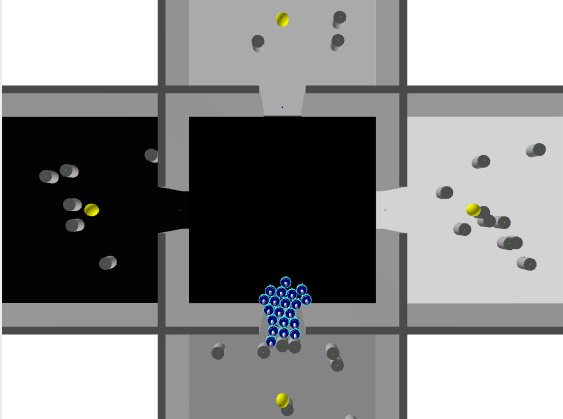
\includegraphics[width=\textwidth]{images/blocked_entrance.png}
        \end{subfigure}%
        ~
        \begin{subfigure}[b]{0.5\textwidth}
                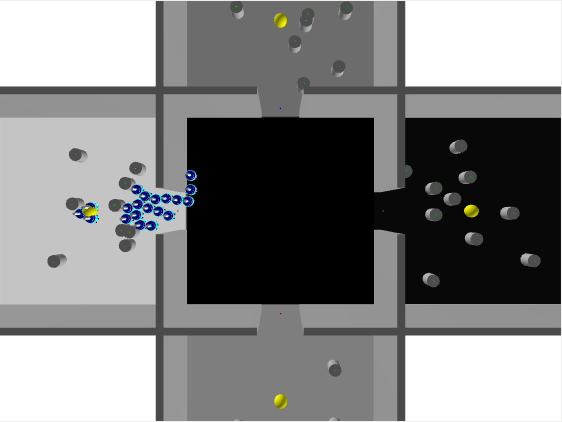
\includegraphics[width=\textwidth]{images/blocked_entrance1.png}
        \end{subfigure}
        \hfill
        \begin{subfigure}[b]{0.5\textwidth}
                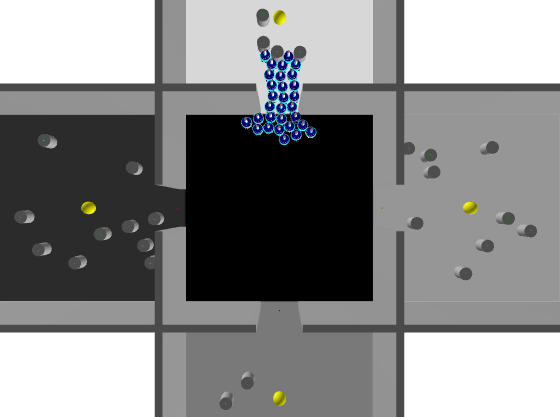
\includegraphics[width=\textwidth]{images/blocked_entrance2.png}
        \end{subfigure}%
        ~
        \begin{subfigure}[b]{0.5\textwidth}
                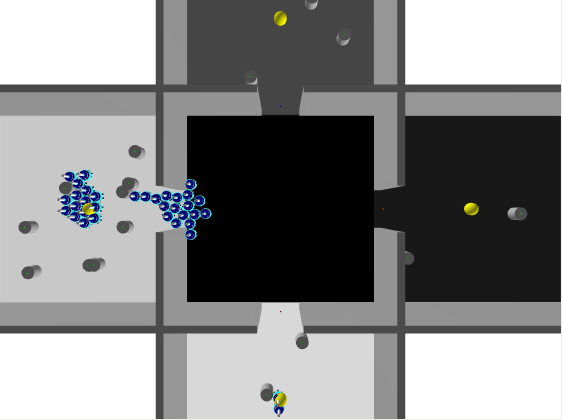
\includegraphics[width=\textwidth]{images/blocked_forces.png}
        \end{subfigure}
        \caption{Blocked robots}\label{fig:blocked}
\end{figure}

% TODO screenshots
